\documentclass[tikz,border=5mm]{standalone}
\usepackage{tikz}
\usetikzlibrary{arrows.meta, positioning, shapes.geometric, calc, patterns}

% --- COLOR DEFINITIONS ---
% Primary
\definecolor{Garnet}{HTML}{73000A}
\definecolor{CGrayDark}{HTML}{555555}
\definecolor{CGrayLight}{HTML}{E5E5E5}
\definecolor{CWhite}{HTML}{FFFFFF}
% Secondary
\definecolor{CRed}{HTML}{CC2E40}
\definecolor{CBlue}{HTML}{466A9F}
\definecolor{CDark}{HTML}{1F414D}
\definecolor{CGreen}{HTML}{65780B}
\definecolor{CLime}{HTML}{CED318}
\definecolor{CGold}{HTML}{A49137}
\definecolor{COrange}{HTML}{D35400}
\definecolor{CPurple}{HTML}{8E44AD}

% --- OBJECT MACROS ---

% Macro to draw the Plane
% #1: Color
\newcommand{\drawPlane}[1]{%
    \begin{scope}[scale=0.06]
         % 1. Fuselage
          \fill[#1] 
            (-4.0, 0) .. controls (-4.0, 0.5) and (-1, 0.6) .. (2.0, 0.45) 
            -- (4.8, 0) -- (2.0, -0.45) 
            .. controls (-1, -0.6) and (-4.0, -0.5) .. (-4.0, 0); 
          % 2. Main Wings
          \fill[#1] 
            (0.8, 0) -- (-1.2, 0) -- (-2.4, 3.2) -- (-1.4, 3.2) -- (1.2, 0) -- cycle;
          \fill[#1] 
            (0.8, 0) -- (-1.2, 0) -- (-2.4, -3.2) -- (-1.4, -3.2) -- (1.2, 0) -- cycle;
          % 3. Horizontal Stabilizers
          \fill[#1] 
            (-2.6, 0) -- (-3.4, 0) -- (-4.4, 1.5) -- (-3.6, 1.5) -- (-2.6, 0) -- cycle;
          \fill[#1] 
            (-2.6, 0) -- (-3.4, 0) -- (-4.4, -1.5) -- (-3.6, -1.5) -- (-2.6, 0) -- cycle;
    \end{scope}
}

% Macro to draw the Quadcopter with guards
% #1: Body/Arm/Guard Color
\newcommand{\drawQuad}[1]{%
    % Elongated central body
    \fill[#1] (0,0) ellipse (0.4 and 0.15);
    
    % Arms connecting to motor mounts
    \draw[#1, line width=1.5pt] (-0.2, 0.05) -- (-0.6, 0.6);
    \draw[#1, line width=1.5pt] (0.2, -0.05) -- (0.6, -0.6);
    \draw[#1, line width=1.5pt] (-0.2, -0.05) -- (-0.6, -0.6);
    \draw[#1, line width=1.5pt] (0.2, 0.05) -- (0.6, 0.6);

    % Define blade and guard style locally
    \def\blade{\fill[CGold, opacity=0.9] (-0.35, -0.03) rectangle (0.35, 0.03);}
    \def\guard{\draw[#1, thin] (0,0) circle (0.4);}

    % Rotors
    \foreach \x/\y/\rotA/\rotB in {-0.6/0.6/45/135, 0.6/-0.6/45/135, -0.6/-0.6/20/110, 0.6/0.6/20/110} {
        \begin{scope}[shift={(\x, \y)}]
            \guard
            \fill[#1] (0,0) circle (0.06); % Motor hub
            \begin{scope}[rotate=\rotA] \blade \end{scope}
            \begin{scope}[rotate=\rotB] \blade \end{scope}
        \end{scope}
    }
}


\begin{document}

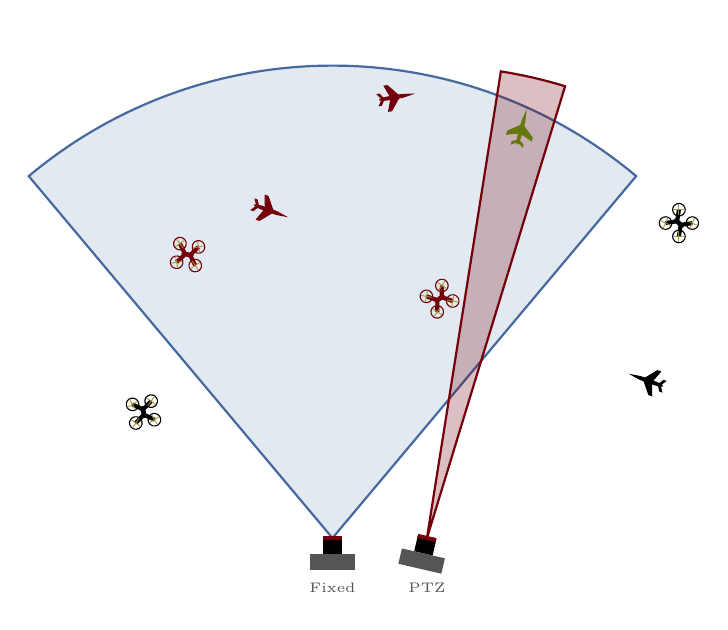
\begin{tikzpicture}[scale=0.8]

    % --- 1. FIELDS OF VIEW ---
    
    % Wide FOV (Blue)
    \begin{scope}
        \coordinate (FixedOrigin) at (-0.5, 0.0);
        \draw[CBlue, thick, fill=CBlue, fill opacity=0.15] 
            (FixedOrigin) -- ++(130:7.5) arc (130:50:7.5) -- cycle;
    \end{scope}
    
    % Zoom FOV (Garnet) - Narrow Beam
    \begin{scope}
        \coordinate (PTZOrigin) at (1.0, 0.0);
        \draw[Garnet, thick, fill=Garnet, fill opacity=0.25] 
            (PTZOrigin) -- ++(81:7.5) arc (81:73:7.5) -- cycle;
    \end{scope}
    
    % --- 2. OBJECTS ---
    
    \def\planeScale{1.1}
    \def\quadScale{0.25}

    % --- Planes ---
    % 1. Original Target Plane (Centered in Zoom FOV) -> GREEN
    \begin{scope}[shift={(2.5, 6.5)}, rotate=75, scale=\planeScale]
        \drawPlane{CGreen}
    \end{scope}

    % 2. Distractor Plane (in Wide FOV, outside Zoom) -> GARNET
    \begin{scope}[shift={(-1.5, 5.2)}, rotate=-20, scale=\planeScale]
        \drawPlane{Garnet}
    \end{scope}

    % 3. Distractor Plane (Outside FOV, bottom right) -> BLACK
    \begin{scope}[shift={(4.5, 2.5)}, rotate=160, scale=\planeScale]
        \drawPlane{black}
    \end{scope}
    
    % 4. Distractor Plane (High center, inside Wide FOV) -> GARNET
    \begin{scope}[shift={(0.5, 7.0)}, rotate=10, scale=\planeScale]
        \drawPlane{Garnet}
    \end{scope}


    % --- Quadcopters ---
    % 1. Original Distractor Quad (in Wide FOV, left) -> GARNET
    \begin{scope}[shift={(-2.8, 4.5)}, rotate=-10, scale=\quadScale]
        \drawQuad{Garnet}
    \end{scope}

    % 2. Distractor Quad (near Zoom FOV edge, inside Wide) -> GARNET
    \begin{scope}[shift={(1.2, 3.8)}, rotate=35, scale=\quadScale]
        \drawQuad{Garnet}
    \end{scope}

    % 3. Distractor Quad (Outside FOV, bottom left) -> BLACK
    \begin{scope}[shift={(-3.5, 2.0)}, rotate=100, scale=\quadScale]
        \drawQuad{black}
    \end{scope}
    
    % 4. Distractor Quad (Far right, outside FOV) -> BLACK
    \begin{scope}[shift={(5.0, 5.0)}, rotate=-45, scale=\quadScale]
        \drawQuad{black}
    \end{scope}

    % --- 3. CAMERAS ---
    
    % Fixed Camera (Left)
    \begin{scope}[shift={(-0.5, 0)}]
        \begin{scope}[rotate=90, scale=0.5]
             \fill[black] (-0.5, -0.3) rectangle (0, 0.3);
             \fill[CGrayDark] (-1, -0.7) rectangle (-0.5, 0.7);
             \draw[Garnet, line width=1.5pt] (0, -0.3) -- (0, 0.3);
        \end{scope}
        \node[below=0.45cm, font=\tiny, color=CGrayDark] {Fixed};
    \end{scope}

    % PTZ Camera (Right)
    % Rotated 77 degrees to align exactly with the target plane
    \begin{scope}[shift={(1.0, 0)}]
        \begin{scope}[rotate=77, scale=0.5]
             \fill[black] (-0.5, -0.3) rectangle (0, 0.3);
             \fill[CGrayDark] (-1, -0.7) rectangle (-0.5, 0.7);
             \draw[Garnet, line width=1.5pt] (0, -0.3) -- (0, 0.3);
        \end{scope}
        \node[below=0.45cm, font=\tiny, color=CGrayDark] {PTZ};
    \end{scope}

\end{tikzpicture}

\end{document}